\section{Results}
\label{sec:accumulator-results}


The benchmark was ran on \gls{hw1} compute-cluster where the client and server parts were distributed in three different ways, namely: within a socket, in two separate sockets of a node and in two separate nodes. Nodes of \gls{hw1} cluster are connected via an  \textit{infiniband} interconnect with the characteristics shown in Figure \ref{fig:hw1-bandwidth}. In order to estimate an effect of pure data accumulation, the benchmark, Listing \ref{lst:bench:auxiliary-subroutines}, was modified to use only blocking \acrshort{mpi} operations i.e. \acrshort{mpi}\_Bcast. We denote the main benchmark as \textit{BM1} and the modified one as \textit{BM2} to distinguish and separately explain effects of non-blocking data transfers and pure data accumulation.\\


Figure \ref{fig:benchmark:results-cube-64} represents results of the benchmarks obtained using \textit{cube-64} communication pattern. The client and server parts of the code were distributed in different sockets within the same node. Factor $F$ was  equal to 1.\\


\begin{figure}[htpb]
\centering
	\begin{tabular}{c}
		\subfloat[A part of \textit{cube-64} communication pattern\label{fig:benchmark:results-comm-pattern}]{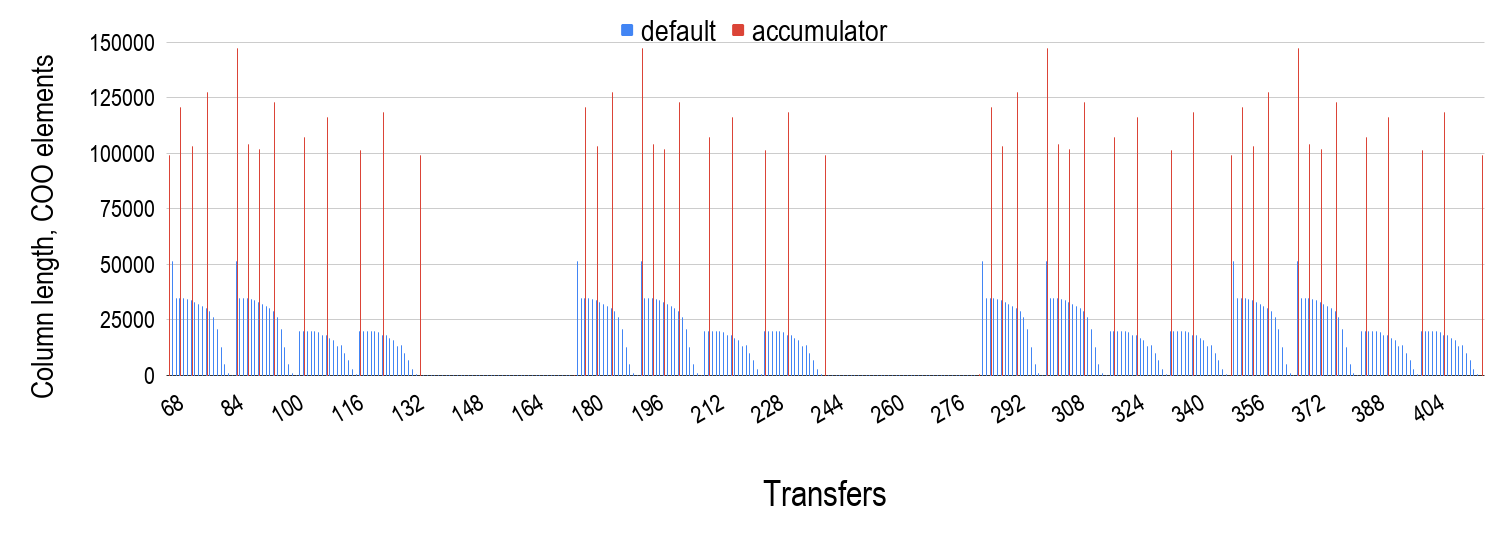
\includegraphics[width=1.0\textwidth]{figures/chapter-3/benchmark-communication-pattern.png}} \\
		\subfloat[BM2: A comparison of the data accumulation concept using blocking communication with the original approach]{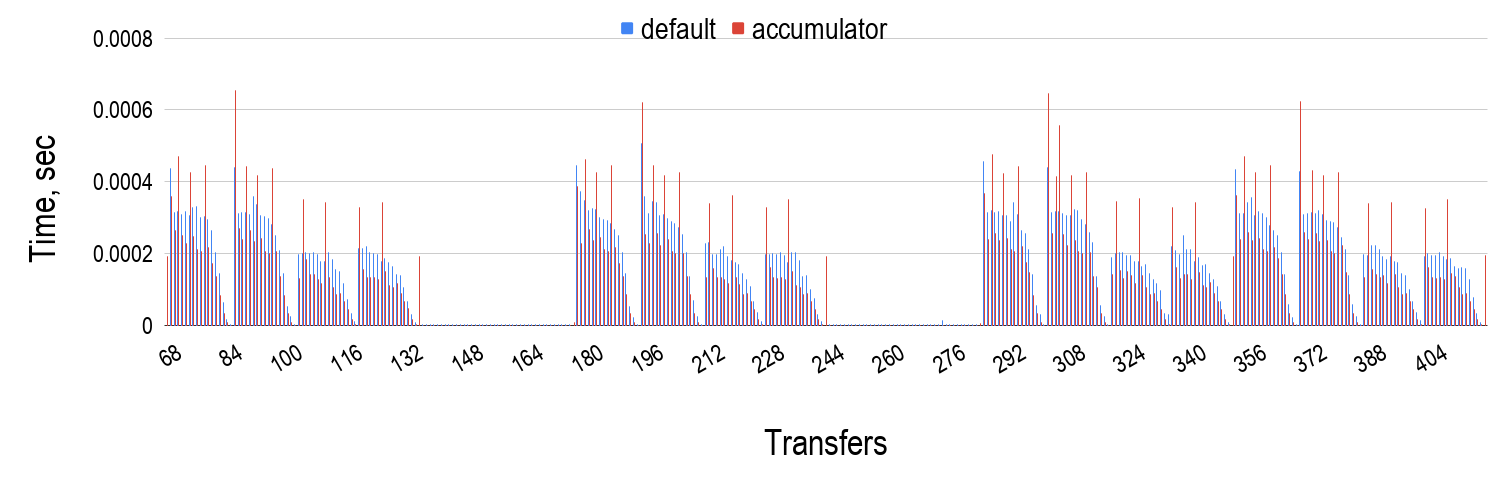
\includegraphics[width=1.0\textwidth]{figures/chapter-3/benchmark-result-blocking.png}} \\
		\subfloat[BM1: A comparison of the data accumulation concept using non-blocking communication with the original approach]{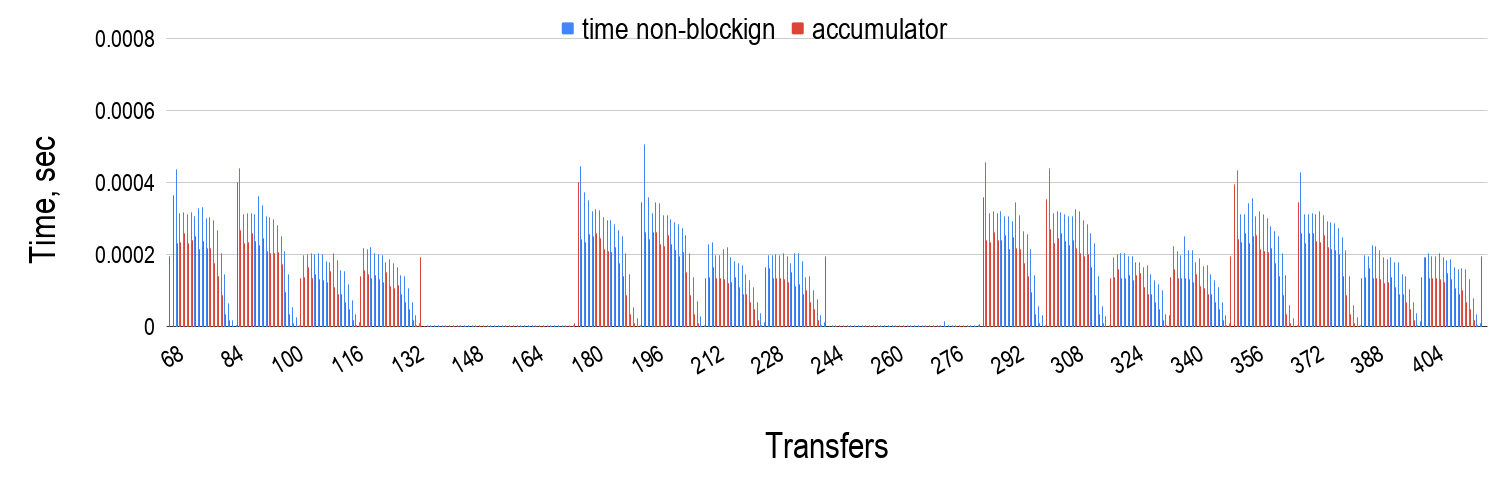
\includegraphics[width=1.0\textwidth]{figures/chapter-3/benchmark-result-non-blocking.png}}
	\end{tabular}
	\caption{Comparisons of the benchmarks running a recorded part of \textit{cube-64} communication pattern between two sockets of a node}
	\label{fig:benchmark:results-cube-64}
\end{figure}


Figure \ref{fig:benchmark:results-comm-pattern} shows that \textit{accumulator} approach results in more than \textbf{6} times drop, from \textbf{344} to \textbf{51}, of the total number of data transfers and resulting resource acquisitions, within the range depicted on the graphs. According to \textit{BM2} benchmark, the accumulation effect reduces the run-time by almost \textbf{9\%} by means of more efficient utilization of intra-node interconnection. The obtained results  also demonstrate that overall, accumulative effect of both accumulation and non-blocking data transfers reduces the run-time of \textit{BM1} benchmark in more than \textbf{26\%}. Table \ref{table:benchmark:performance-gain} summarizes results obtained for all three client-server distributions within the same range of the recorded communication pattern displayed in Figure \ref{table:benchmark:performance-gain}.\\


\begin{table}[ht]
\centering
\begin{tabular}{|c|c|c|}
\hline
\begin{tabular}[c]{@{}c@{}}Benchmark\\ name\end{tabular} & BM2, \% & BM1, \% \\ \hline
within a socket                                          & 7.61    & 13.84   \\ \hline
between sockets                                          & 9.04    & 26.26   \\ \hline
between nodes                                            & -2.06   & 3.20    \\ \hline
\end{tabular}
\caption{Time reduction of data transfers with respect to the original implementation in case of execution of \textit{cube-64} communication pattern}
\label{table:benchmark:performance-gain}
\end{table}


It turns out that \textit{BM2} benchmark is slower than the original \acrshort{athlet} approach in  approximately \textbf{2\%} in case of  inter-node communication. However, non-blocking data broadcasts, according to \textit{BM1} benchmark, help to alleviate the slow-down and achieve almost \textbf{3\%} of improvement.\\


Unimpressive results of non-blocking  inter-node communication can be explained by specifics of the benchmark design. In particular, time spent on generation of random matrix elements was not enough to overlap time spent on non-blocking data transfers in case of \textit{cube-64} test-case, see Figure \ref{fig:benchmark:results-cube-64-inter-node-comm}. Hence, the execution control was probably suspended by \acrshort{mpi} library at each subsequent call of \textit{MPI\_Wait()} function.\\


\begin{figure}[htpb]
  \centering
  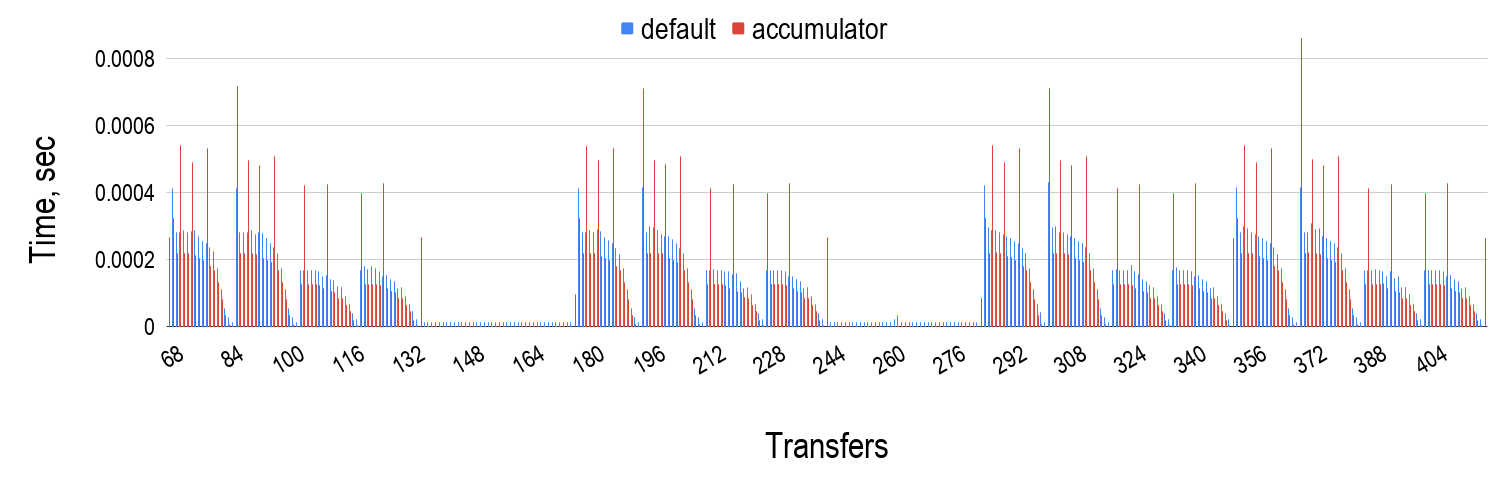
\includegraphics[width=1.0\textwidth]{figures/chapter-3/benchmark-result-non-blocking-inter-node-comm.png}
  \caption{A comparison of \textit{BM1} benchmark with the original implementation running a recorded part of \textit{cube-64} communication pattern between two compute-nodes}
\label{fig:benchmark:results-cube-64-inter-node-comm}
\end{figure}


The slow-down resulting from pure data accumulation could be explained by automatic \acrshort{mpi} protocol switching, namely: \textit{Eager} and \textit{Rendezvous} \cite{mpi:protocols-explanation}. The protocols are dedicated to small and large message transfers, respectively, where a quantitative measure of the message size is defined by a concrete implementation of the \acrshort{mpi} standard, however, it can be controlled through dedicated environment variables.\\



Similar results were observed for \textit{cube-645} test case where the number of equations was approximately $\bm{10^6}$ and the average compressed Jacobian column length reached around $\bm{1.7 \cdot 10^5}$ elements. In case of  inter-node communication, \textit{BM1} benchmark again showed performance degradation by \textbf{6.35\%} whereas non-blocking data broadcasts improved run-time by \textbf{23.21\%}. Such performance jump, from \textbf{-6.35\%} to \textbf{23.21\%}, can be explained by the fact that time spent on generation of random elements was enough to hide the corresponding data transfers and overheads.\\



Ideas, expressed in \textit{BM1} benchmark, Listings \ref{lst:bench:auxiliary-subroutines} and \ref{lst:beanch:pseudocode}, were successfully implemented in \acrshort{nut}, namely: in the client side of \acrshort{nut} located in \acrshort{athlet}. Several simulation scenarios were taken for the final verification and performance testing, namely: \textit{cube-64}, \textit{k3-2} and \textit{pwr-3d}. Verification of the modified code did not detect any deviations of numerical results from the original implementation. Additionally, all tests showed considerable improvements in communication time. As an example, time spent on communication between \acrshort{athlet} and \acrshort{nut} during compressed Jacobian transfers decreased by \textbf{66.17\%}, \textbf{76.03\%} and \textbf{42.55\%} for intra-socket, intra-node and inter-node client-server process allocations, respectively, for \textit{pwr-3d} scenario, taking it as the most representative simulation test-scenario known in \acrshort{grs}. However, the overall improvement of applied changes achieved only \textbf{0.14\%} on average, regardless of a client-server allocation. Profiling showed the communication part of the original implementation took around \textbf{0.24\%} of the total time spent on matrix evaluations and transfers. This fact explains this negligible overall performance gain, resulted from the source code modification, that was observed in all conducted final tests.\\
